\documentclass[]{article}
\usepackage[T1]{fontenc}
\usepackage[utf8]{inputenc}
\usepackage[polish]{babel}
\usepackage{enumitem}
\usepackage{graphicx}
%\usepackage[top=1in, bottom=1in, left=1in, right=1in]{geometry}

\title{Phishing}
\author{Nikodem Kaczmarek, Patryk Garwol}

\begin{document}
\maketitle

\newpage 

\section{Wprowadzenie}
 \cite{whatIsPhishingCNBC}


\newpage
\section{Mechanizm działania phishingu}

Phishing przypomina słowo fishing, w szczególności gdy skupimy się na wymowie. Nie jest to przypadek, ponieważ ataki tego rodzaju są w pewien sposób "łowieniem rybek" \cite{govpl_phishing}:
\begin{itemize}[label=$\rightarrow$]
	\item wędkarz - przestępca
	\item przynęta - wiadomość, szkodliwy link, fałszywa strona itp.
	\item ryba - zasoby nieświadomej ofiary
\end{itemize} 

Mowa tutaj zatem o inżynierii społecznej, czyli technice manipulacji, która wykorzystuje ludzkie błędy w celu uzyskania prywatnych informacji lub innych zasobów \cite{kaspersky_social_engineering}.
Zdarzają się również przypadki, w których przestępca jest na tyle złośliwy, że wykorzystując phishing instaluje na sprzęcie ofiary złośliwe oprogramowanie, które niekoniecznie służy do kradzieży danych. Oszustwa te wykorzystują najsłabsze ogniwo w świecie informatyki, czyli człowieka. Większość populacji, w szczególności osoby starsze - nie jest obeznana w kwestii informatyki \cite{dsgi_wiley}, nie mówiąc już o cyberbezpieczeństwie. Łatwo jest wykorzystać ich niewiedzę, co w połączeniu z socjotechnikami daje atakującym dużo pola do popisu w kwestii doboru ich "przynęty".

Atak phishingowy może zostać przeprowadzony na nieokreślonych ofiarach. Atakujący wówczas liczą, że ktokolwiek "złapie się na haczyk". W dobie internetu bardzo łatwo jest wysyłać e-maile, lub nawet sms-y do niezliczonej liczby osób. Próg wejścia do zautomatyzowania takich procesów jest bardzo niski i ofiara nie potrzebuje lat nauki programowania, żeby do takiego ataku doprowadzić, ponieważ wystarczy zainstalować na komputerze IDE Pythona, a następnie poświęcić 5 sekund życia, aby znaleźć odpowiedni przewodnik, na przykład "How to Send Automated Email Messaged in Python" opublikowany w witrynie geeksforgeeks.org \cite{geeks4geeks_automaticmails}. Czyni to ten proceder bardziej przerażającym, wiedząc jak proste jest to przedsięwzięcie. Zdecydowana osób nie nabierze się na e-mail przysłowiowego Księcia z Nigerii \cite{nigerian_prince}. Jest jednak procent ludzi, które są podatne na ataki tego typu.

Groźniejszym rodzajem phishingu jest spear-phishing. Polega on na zaatakowaniu określonej osoby lub podmiotu, co rażąco wpływa na jego skuteczność. Ataki te są planowane dłuższy czas, aby dokładnie poznać słabe strony ofiary i tym sposobem zoptymalizować szanse powodzenia. Według raportu firmy Proofpoint z roku 2020, w roku 2019. 88\% organizacji na świecie doświadczyło zagrożenia tego rodzaju. Spośród nich aż 55\% stało się jego ofiarami \cite{proofpoint2020}.

\begin{figure}
	\centering
	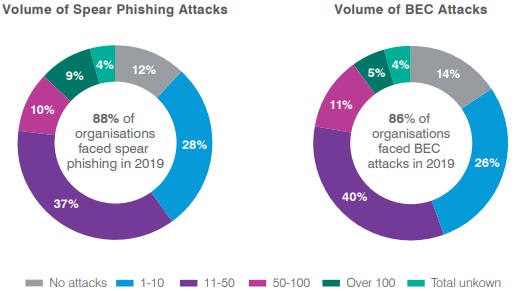
\includegraphics[width=0.8\linewidth]{Pictures/proofpoint_phishing2019.jpg}
	\caption{Skala ataków phishingowych w 2019. roku wg. raportu Proofpoint}
	\label{fig:sample}
\end{figure}

\newpage
\section{Narzędzia i techniki wykorzystywane przez oszustów}

\newpage
\section{Cele ataków phishingowych}

\newpage
\section{Sposoby identyfikacji phishingu}

\newpage
\section{Skutki ataków phishingowych}

\newpage
\section{Ochrona przed phishingiem}

\newpage
\section{Studium przypadku: Znane ataki phishingowe}

\newpage
\section{Przyszłość phishingu}

\newpage
\section{Podsumowanie}

\newpage
\bibliographystyle{plain}
\bibliography{bibliografia.bib}
\end{document}
